\documentclass[18pt, aspectratio=169]{beamer}
% \documentclass{etp-beamer-fancy}
\usepackage[utf8]{inputenc}
% \usepackage{templates/mytemplate}
\usepackage{templates/beamerthemekit}
\usepackage{graphicx}
\usepackage{microtype}
\usepackage{xcolor}
\usepackage{hyperref}
\usepackage{siunitx}
\usepackage{upgreek}
\usepackage{hepnames}
\usepackage{appendixnumberbeamer}
\usepackage{booktabs}
\NewDocumentCommand\angrange{O{} m m}{\SIrange[parse-numbers=false,#1]{\ang[parse-numbers=true]{#2}}{\ang[parse-numbers=true]{#3}}{}}
\usepackage{subcaption}
% \usepackage{enumitem}

\title{MVA Track Quality Estimation for the Belle II Experiment}
\subtitle{DPG Frühjahrstagung 2019}
\author[Michael Eliachevitch (\href{mailto:michael.eliachevitch@kit.edu}{michael.eliachevitch@kit.edu})]{F.~Bernlochner, N.~Braun,
  \underline{M.~Eliachevitch (\href{mailto:michael.eliachevitch@kit.edu}{michael.eliachevitch@kit.edu})}, F.~Metzner}
\titleimage{tracks_wide}
\titlelogo{belle2-logo}
\institute[ETP -- KIT]{Institut für Experimentelle Teilchenphysik (ETP) -- KIT}
\date{27 March 2019}

\newcommand{\kitemph}[1]{\textcolor{kit-green100}{\bf{#1}}}

\begin{document}

\selectlanguage{english}
\begin{frame}
  \titlepage
\end{frame}
\begin{frame}
  \frametitle{The Belle II Detector}
  \begin{center}
    \includegraphics<1>[width=.75\textwidth]{figures/belle2_detector_dpgaachen.pdf}
    \includegraphics<2>[width=.75\textwidth]{figures/belle2_detector_dpgaachen_highlighted.pdf}
  \end{center}
\end{frame}
\begin{frame}

  \frametitle{Tracking subdetectors}
  \begin{columns}[t]
    \begin{column}{.5\textwidth}
      \center
      CDC wire arrangement
      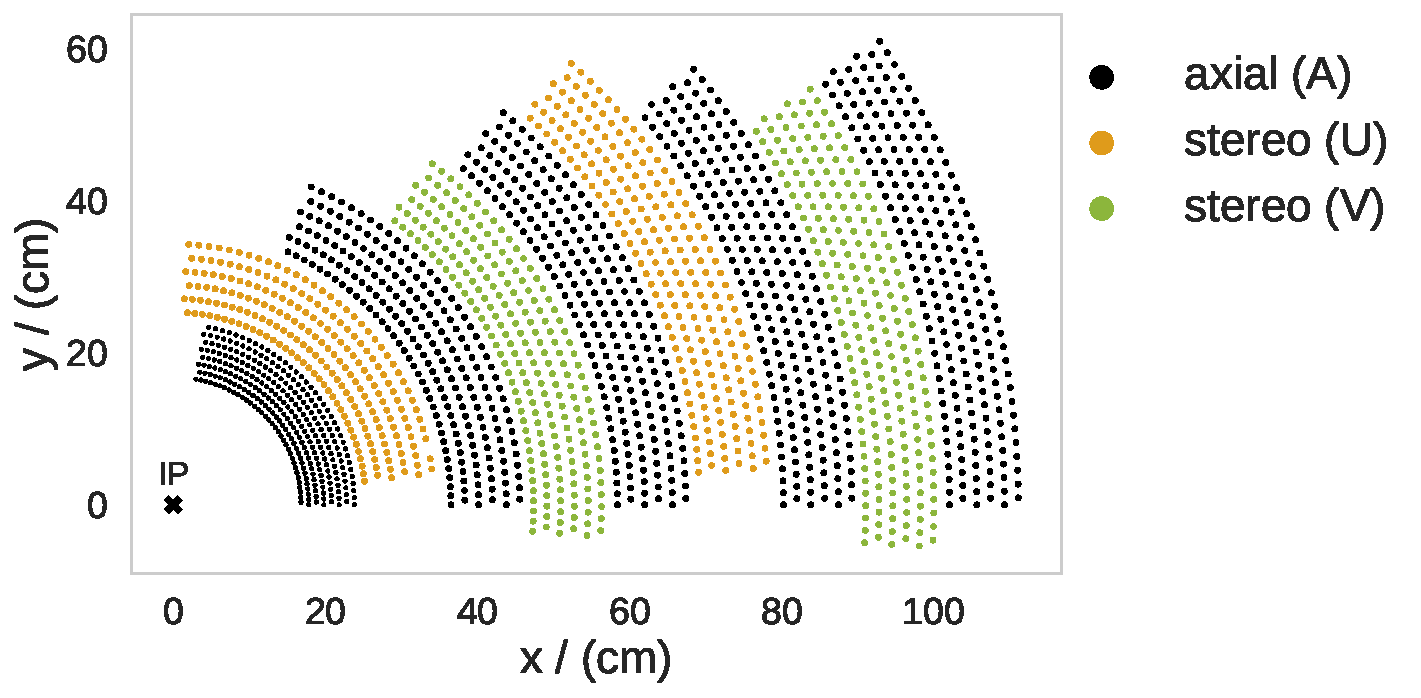
\includegraphics[width=.9\textwidth]{figures/my_cdc_wire_configuration_plot.pdf}
      % 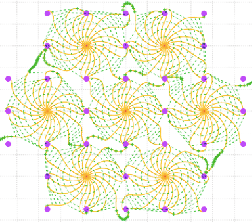
\includegraphics[width=.5\textwidth]{figures/drift_cells_isochrones.png}
      \begin{columns}[t]
        \begin{column}{.4\textwidth}
          \center
          axial layer
          \includegraphics[width=\textwidth]{figures/axial_layer_cropped.pdf}
        \end{column}
        \begin{column}{.4\textwidth}
          \center
          stereo layer
          \includegraphics[width=\textwidth]{figures/stereo_layer_hyperboloid_cropped.pdf}
        \end{column}
      \end{columns}
    \end{column}
    \begin{column}{.5\textwidth}
      \center
      VXD\\
      \includegraphics[width=.5\textwidth]{figures/vxd_layers_labelled.png}\\
      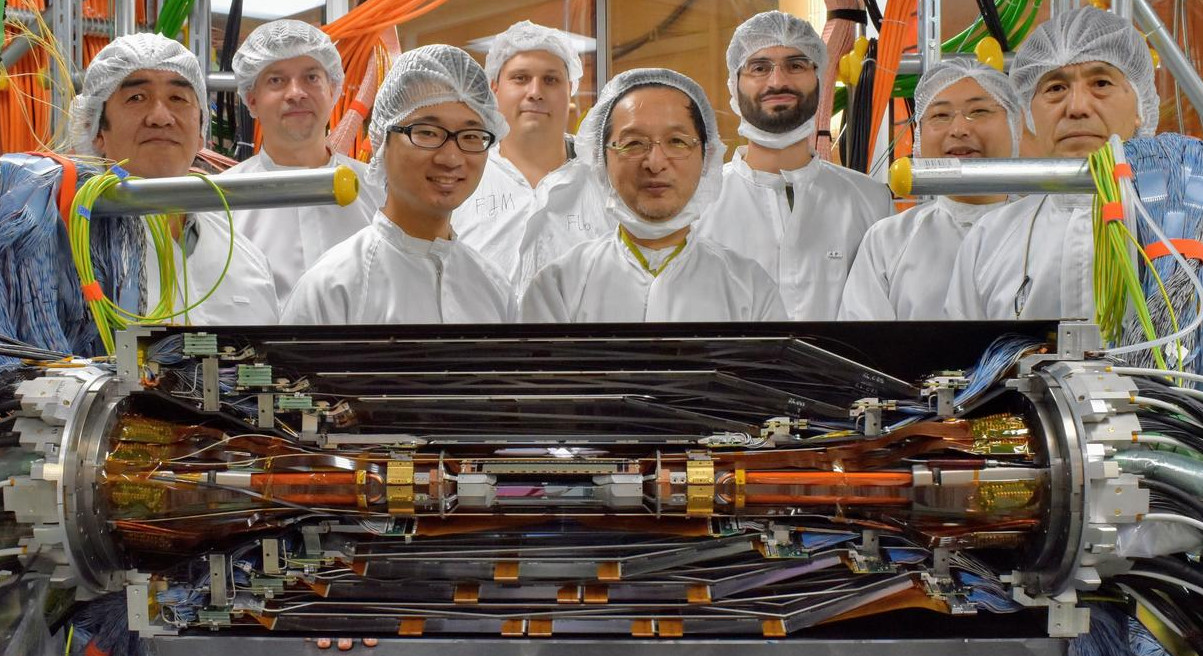
\includegraphics[width=.65\textwidth]{figures/vertexdetector_cropped.jpg}
    \end{column}
  \end{columns}
\end{frame}
\begin{frame}
  \frametitle{Tracking Challenges at Belle II}
  \begin{columns}
    \begin{column}{0.5\textwidth}
      \begin{itemize}
      \item \textcolor{kit-blue100}{$\sim$\textbf{11} tracks} per $\Upupsilon(\text{4S})$ decay event, but\ldots
      \end{itemize}
      \begin{alertblock}{Challenges}
        \begin{itemize}
        \item low-momentum tracks
        \item large beam-induced backgrounds
        \item e.g.\ PXD: \textcolor{kit-red100}{$\mathcal{O}({\bf 10^4})$ background hits}
        \item yet: many Belle~II analyses requires high efficiency/purity
        \end{itemize}
        % \begin{figure}
        %   \centering
        %   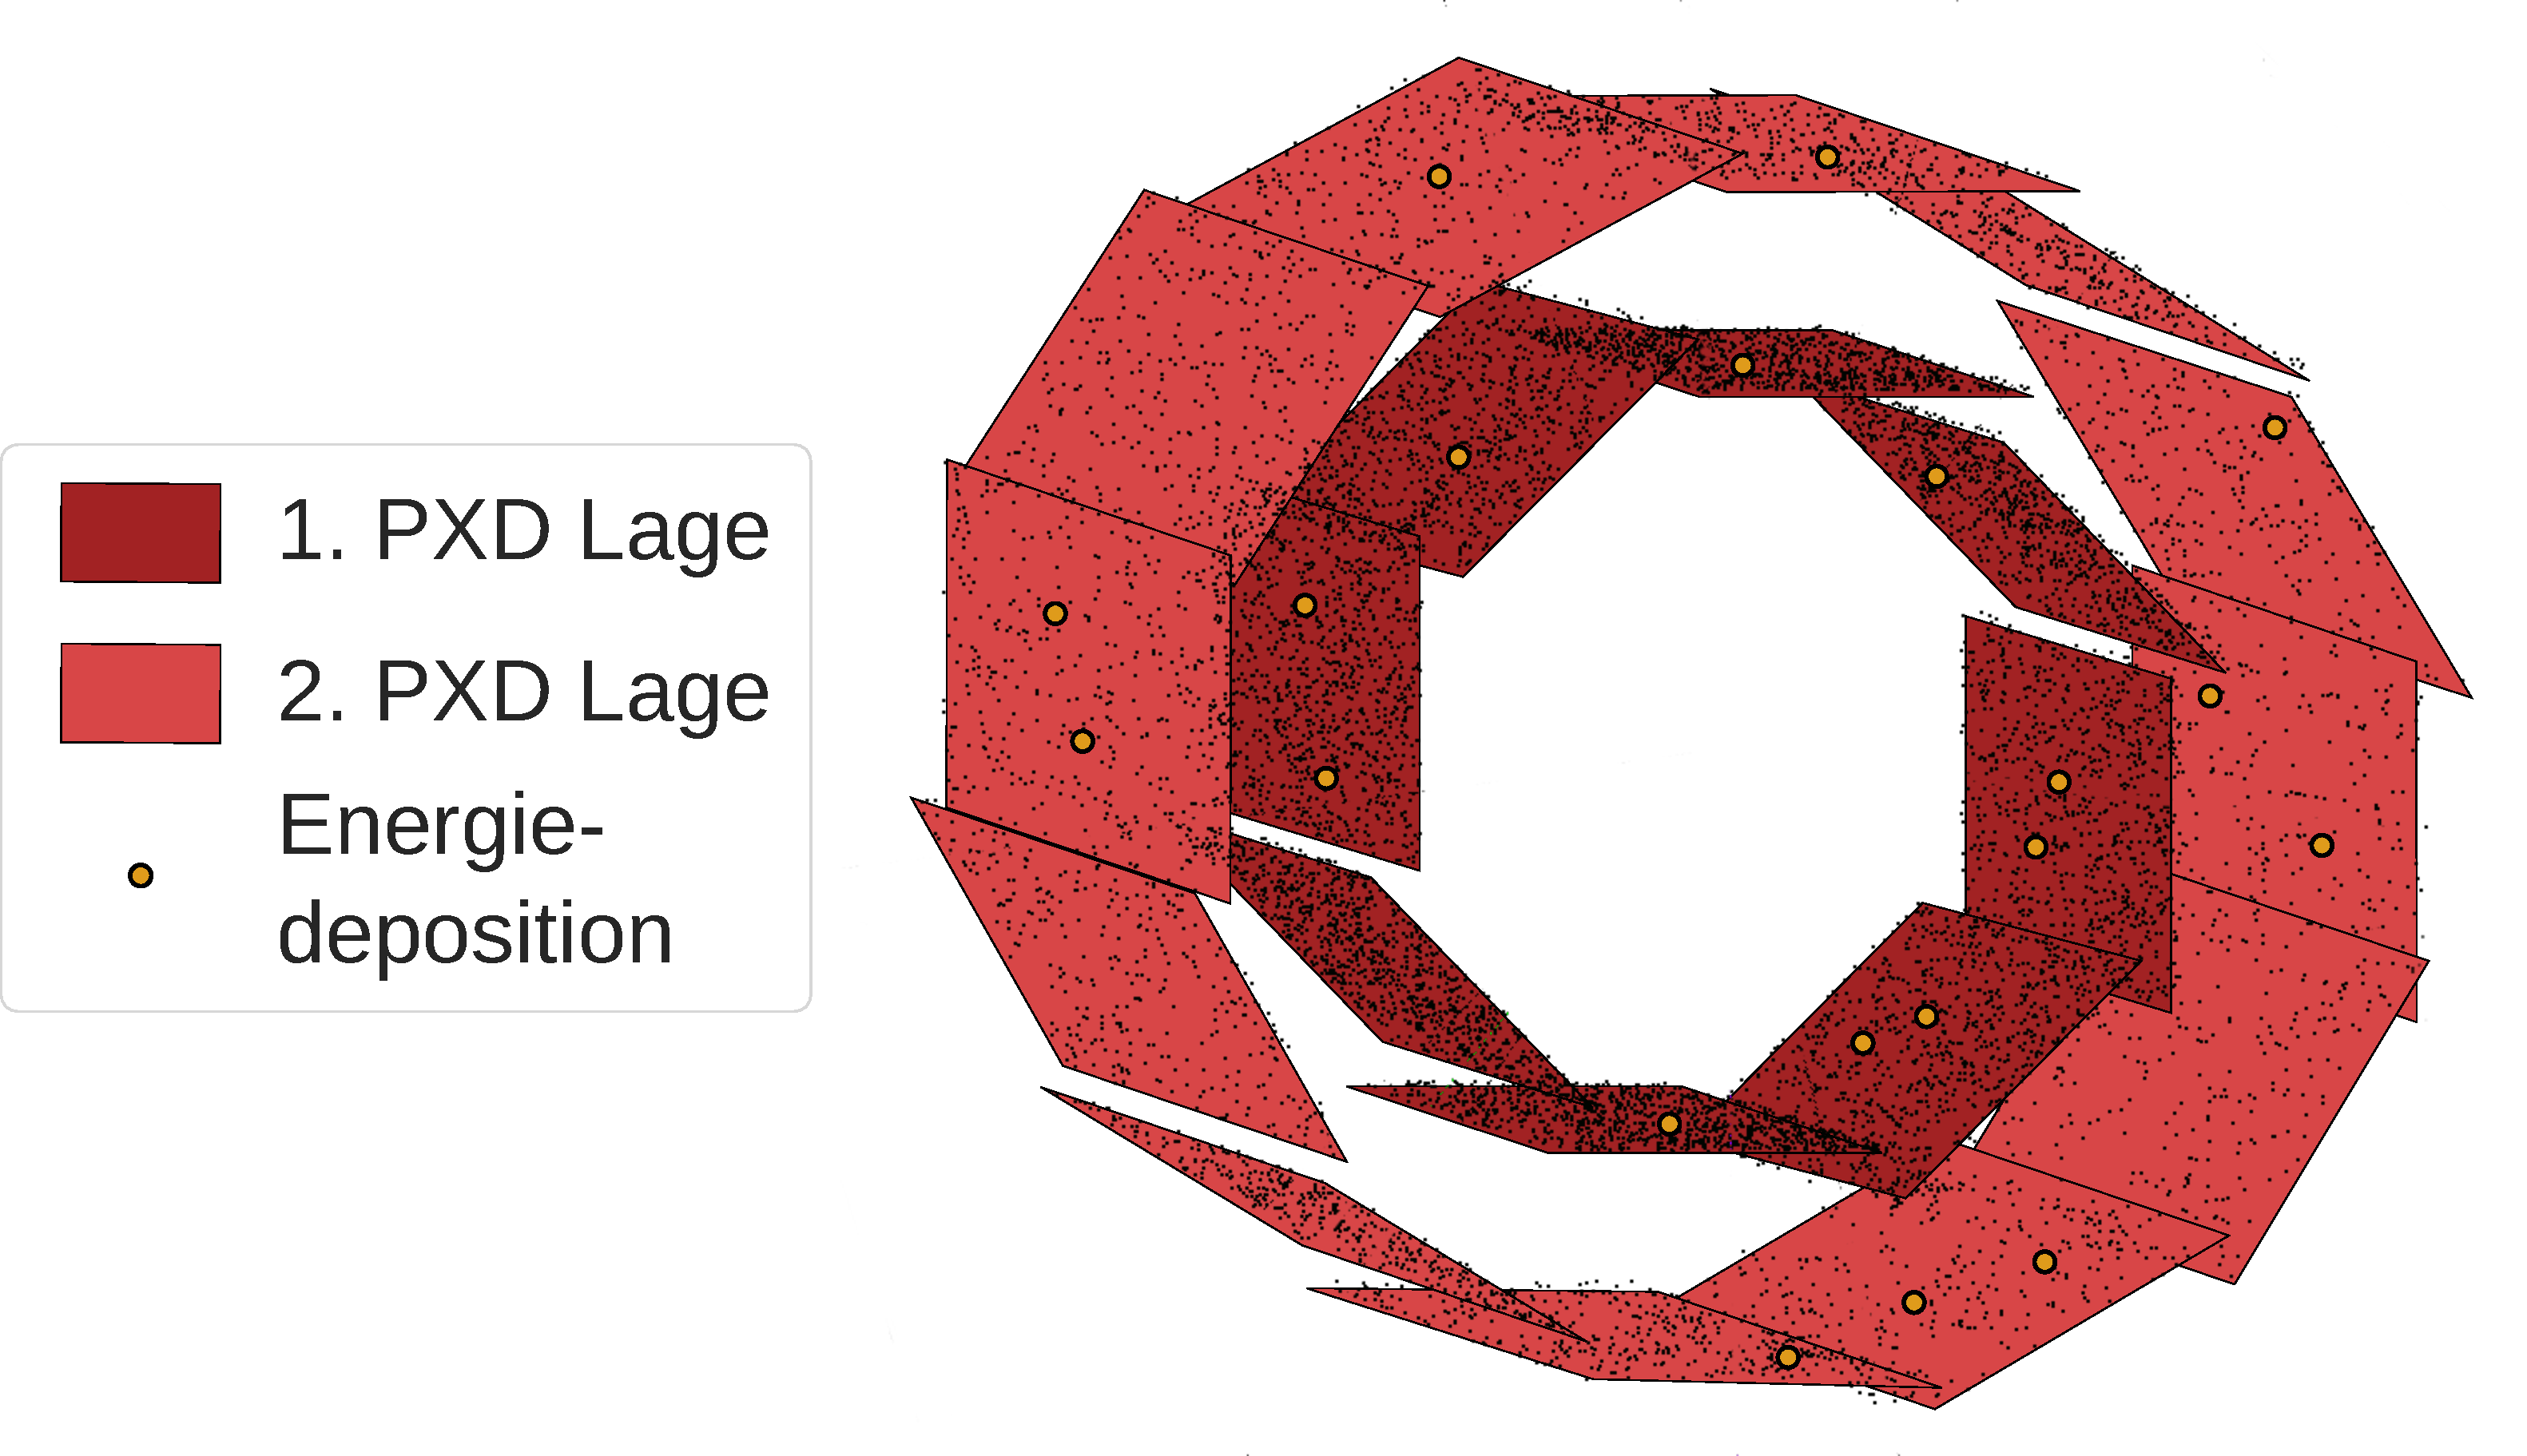
\includegraphics[width=.5\textwidth]{figures/background_colored.pdf}
        % \end{figure}

      \end{alertblock}
      \begin{block}{Solution}
        \begin{itemize}
        \item multiple subdetectors
        \item and respective tracking algorithms
        \end{itemize}
      \end{block}
    \end{column}
    \begin{column}{0.5\textwidth}
      \centering
      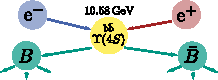
\includegraphics[width=.7\textwidth]{figures/eplus_eminus_to_b_bar_diagram.pdf}\\
      % \includegraphics[width=0.7\textwidth]{figures/first_y4s.jpg}
      \includegraphics[width=.7\textwidth]{figures/b2phase3_1st_bantib_like_event_cropped.png}\\
      \scriptsize (first \PB{}\APB-collision with full 2019 geometry)
    \end{column}
  \end{columns}
\end{frame}
\begin{frame}
  \frametitle{Belle II Track Reconstruction Chain}
  \begin{columns}
    \begin{column}{0.53\textwidth}
      \begin{itemize}
      \item \kitemph{CDC standalone} track finding\\
        based on the global Legendre transform (extended Hough)
      \item \kitemph{SVD standalone} track finding\\
        uses a cellular automaton algorithm
      \item \kitemph{Combinatorial Kalman Filter (CKF)}\\
        extrapolate from existing tracks to attach tracks/hits in other subdetectors and
        do track merging
      \item \textbf{\textcolor{kit-blue100}{track fitting}}\\
        at the end to extract track parameters \
      \end{itemize}
    \end{column}
    \begin{column}{0.47\textwidth}
      \centering
      \includegraphics[width=.95\textwidth]{figures/full_track_finding_simplified.pdf}
    \end{column}
  \end{columns}
\end{frame}

\begin{frame}
  \frametitle{Finding Efficiency vs. Purity}
  \begin{block}{Figures of merit}
    \begin{itemize}
    \item \textbf{finding efficiency: \SI{96.1}{\percent}}\\
      ratio of found MC tracks
    \item \textbf{fake rate: \SI{2.4}{\percent}}\\
      ratio of pattern recognition tracks not corresponding to an MC track
    \item \textbf{clone rate: \SI{6.9}{\percent}}\\
        ratio of pattern recognition tracks corresponding to an already found MC track
    \end{itemize}
  \end{block}
  \begin{itemize}
  \item Tuning the tracking reconstruction is requires a \kitemph{trade-off}:\\
    finding efficiency vs. fake and clone rates
  \end{itemize}
\end{frame}
\begin{frame}
  \frametitle{Track Quality Indicator}
  \begin{itemize}
  \item Goal: Enable physics analysts to \kitemph{choose working point} on the efficiency vs.
    purity receiver operating curve (ROC)
  \item assign a \kitemph{quality indicator (QI)} to the final tracks
  \item include low-level \kitemph{tracking information} in addition to already existing information from the fit (e.g.\ $\chi^2$), 
  \item Solution: Train an multivariate (MVA) classifier $=$ \kitemph{track quality estimator}
  \end{itemize}
    \begin{block}{MVA Algorithm: FastBDT\footnote[frame]{Keck, T. (2017) FastBDT: a Speed-Optimized
        Multivariate Classification Algorithm for the Belle II Experiment}}
    \begin{itemize}
    \item a stochastic gradient-boosted decision tree
    \item prevent over-fitting via multiple shallow decision trees (\emph{boosted}) and random sub-samples of training data
      (\emph{stochastic})
    \item high speed via equal-frequency binning of inputs and cache-friendly memory access
    \end{itemize}
  \end{block}
\end{frame}
\begin{frame}
  \frametitle{Features for Training the Quality Estimator}
    \begin{itemize}
    \item training target: MC truth to discriminate fake (and clone) from correct tracks in training
    \item input variables: use all information available during the reconstruction
    \item \kitemph{intermediate quality estimators} for the individual track finders
      \begin{itemize}
      \item many features only available to the tracking algorithms in the subdetectors, e.g.
      \item CDC: drift lengths, ADC signal size, individual hit pattern, \ldots
      \item SVD: deposited charge, number of clusters, individual hit pattern, \ldots
      \end{itemize}
    \item hit patterns and hit weights from the track fit
    \item momentum and positional information
    \item timing information
    \item merger information from the CKF ($\chi^2$)
    \item \ldots
    \end{itemize}
\end{frame}

\begin{frame} 
  \frametitle{Example Feature Distributions}
  \begin{columns}[t]
    \begin{column}{.5\textwidth}
      \center
      From CDC tracking: e.g.\ drift lengths
      \includegraphics[width=\textwidth]{figures/cdc-qi-new/drift_length_sum.pdf}
    \end{column}
    \begin{column}{.5\textwidth}
      \center
      From fit: e.g.\ track-parameters
    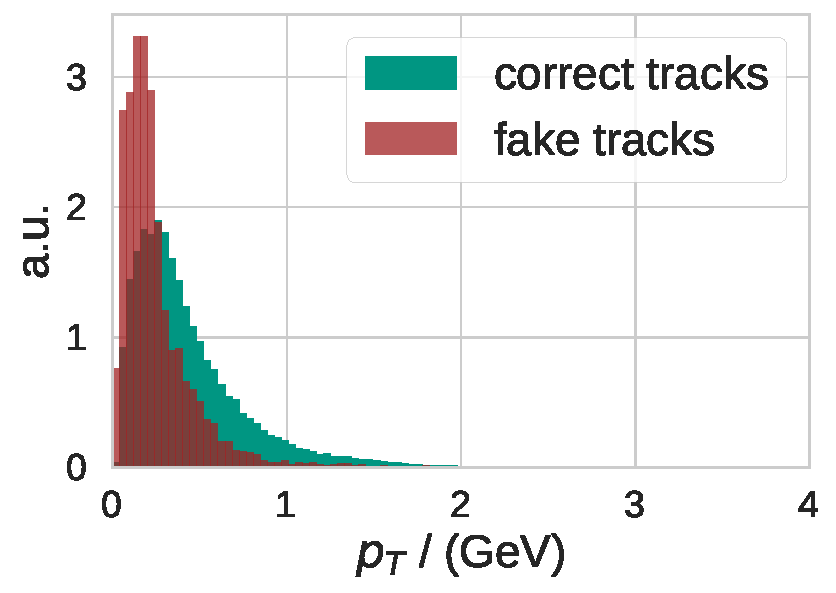
\includegraphics[width=\textwidth]{figures/combined-qi/pt_distributions.pdf}
    \end{column}
  \end{columns}
  
\end{frame}

\begin{frame}
  \frametitle{Performance of Quality Estimators in the SVD and VXD}
  \begin{columns}
    \begin{column}{.5\textwidth}
      \center
      SVD Quality Indicator ROC\\
      % 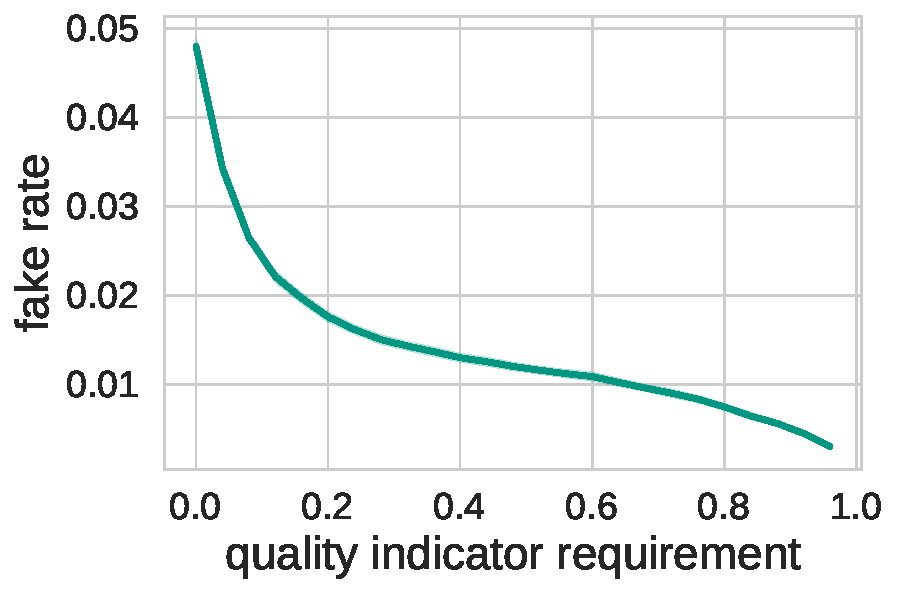
\includegraphics[width=.5\textwidth]{figures/vxd-qi/fake_rate.pdf}
      \includegraphics[width=.9\textwidth]{figures/vxd-qi/roc_curve.pdf}
    \end{column}
    \begin{column}{.5\textwidth}
      \center
      CDC Quality Indicator ROC\\
      % 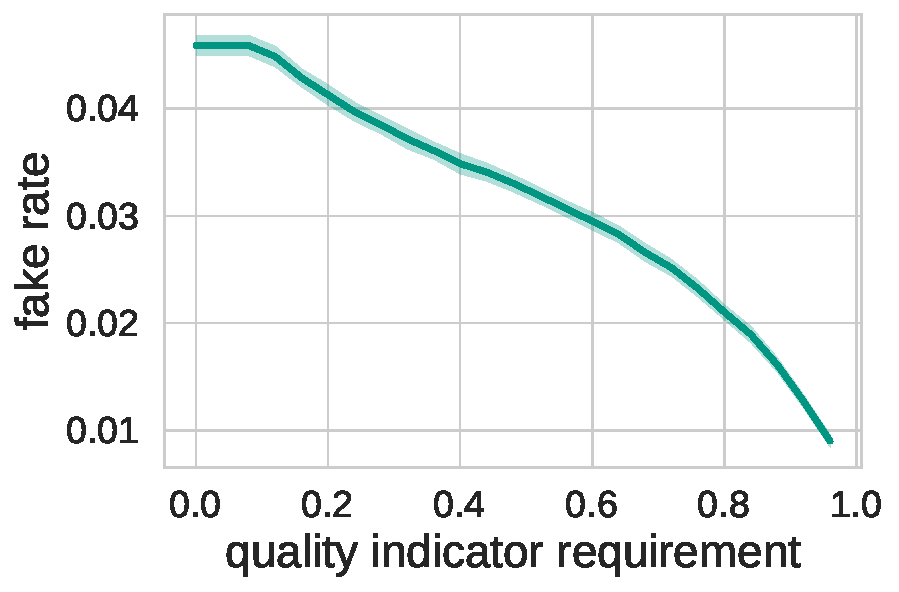
\includegraphics[width=.5\textwidth]{figures/cdc-qi-new/fake_rate.pdf}
      \includegraphics[width=.9\textwidth]{figures/cdc-qi-new/roc_curve.pdf}
    \end{column}
  \end{columns}
  \begin{block}{}
  good separation of fake tracks in the individual track finders\\
  $\Rightarrow$~feed quality indicators into combined quality estimation
  \end{block}

\end{frame}
\begin{frame}
  \frametitle{Performance of Combined Quality Estimation (preliminary)}
  \begin{columns}
    \begin{column}{.65\textwidth}
      \center
      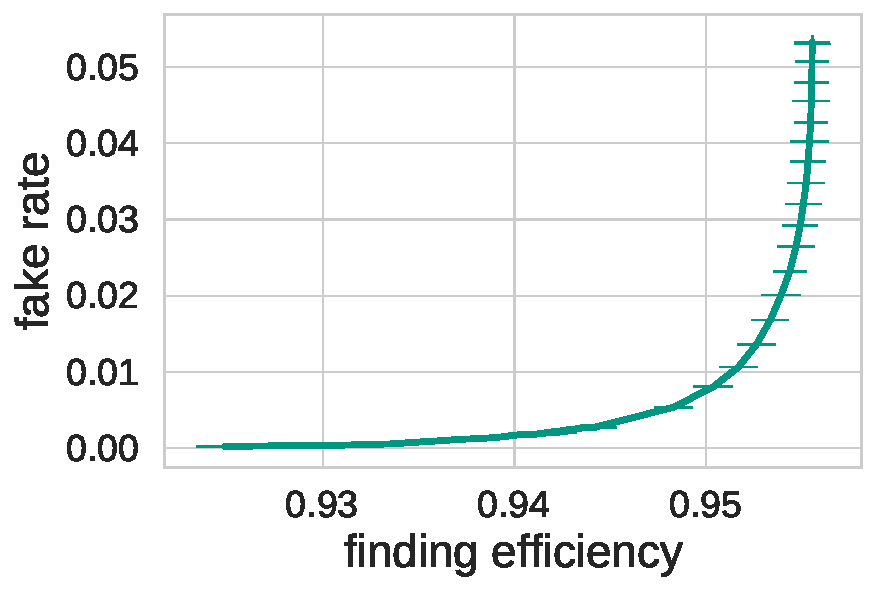
\includegraphics[width=.8\textwidth]{figures/combined-qi/fullqi_roc_curve.pdf}
      \begin{block}{}
        combined features of all track finders yield good fake suppression with only small finding
        efficiency losses
      \end{block}


    \end{column}
    \begin{column}{.35\textwidth}
      \center
      \includegraphics[width=\textwidth]{figures/combined-qi/fullqi_fake_rate.pdf}
      \includegraphics[width=\textwidth]{figures/combined-qi/fullqi_findeff.pdf}
    \end{column}
  \end{columns}
\end{frame}
\begin{frame}
  % \frametitle{Summmary}
  \begin{block}{Summary}
    \begin{itemize}
    \item quality estimator can utilize information from different track finders to
      classify fake tracks well
    \item quality indicator is included in the final tracks and will provide a useful tool for many
      analyses
    \item further work can be done to include and study more input variables and do a
      hyper-parameter optimization for the MVA method used
    \end{itemize}
  \end{block}

  \vspace{3cm}
  \Large Thank you for your attention.
\end{frame}

\appendix
\backupbegin

\begin{frame}
  \centering \huge
  Backup
\end{frame}

\begin{frame}
  \frametitle{Technical Parameters of the CDC}
  \begin{table}
    \centering
    % \caption{\label{tab:cdc-param}Technical parameters of the Belle~II central drift
    % chamber. The values are taken from~\cite{Abe:2010gxa}.}
    \begin{tabular}{lc}
      \toprule
      Parameter                                & Value                                                 \\
      \midrule
      gas mixture                              & \SI{50}{\percent} He  -- \SI{50}{\percent}
                                                 C$_2$H$_6$ \\

      $X/X_0$ at $\theta = \ang{90}$           & \SI{2.5}{\percent}                      \\
      radius of the inner cylinder             & \SI{16.0}{\cm}                          \\
      radius of the outer cylinder             & \SI{113.0}{\cm}                         \\
      radius of the innermost layer            & \SI{16.8}{\cm}                          \\
      radius of the outermost layer            & \SI{111.14}{\cm}                        \\
      polar acceptance                         & \angrange{17}{150}                      \\
      number of superlayers                    & 9 (5 axial, 4 stereo)                   \\
      % superlayer configuration                                                         \\
      % (A: axial, U: pos. skew, V: neg. skew) & A-U-A-V-A-U-A-V-A                       \\
      number of layers                         & 56 (8 in first superlayer, 6 in others) \\
      number of sense wires                    & \num{14336}                             \\
      diameter of sense wires                  & \SI{30}{\micro\meter}                   \\
      \bottomrule
    \end{tabular}
  \end{table}
\end{frame}

\begin{frame}
  \frametitle{CDC drift cell configuration}
  \center
  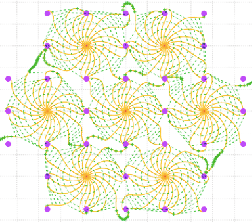
\includegraphics[width=.5\textwidth]{figures/drift_cells_isochrones.png}
\end{frame}

\begin{frame} 
  \frametitle{Finding efficiency and Fake Rate for the CDC QE}
  \begin{columns}
    \begin{column}{.5\textwidth}
      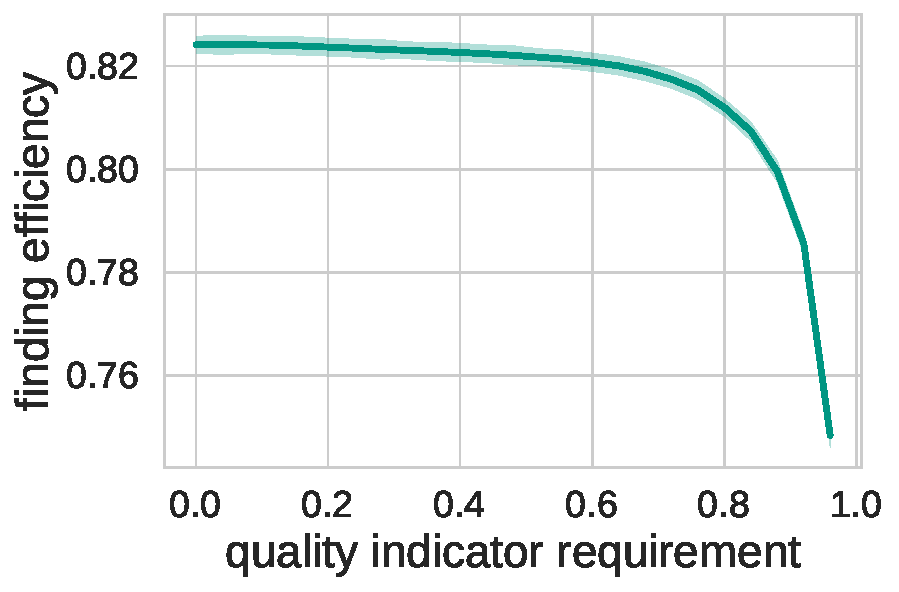
\includegraphics[width=\textwidth]{figures/cdc-qi-new/findeff.pdf}
    \end{column}
    \begin{column}{.5\textwidth}
      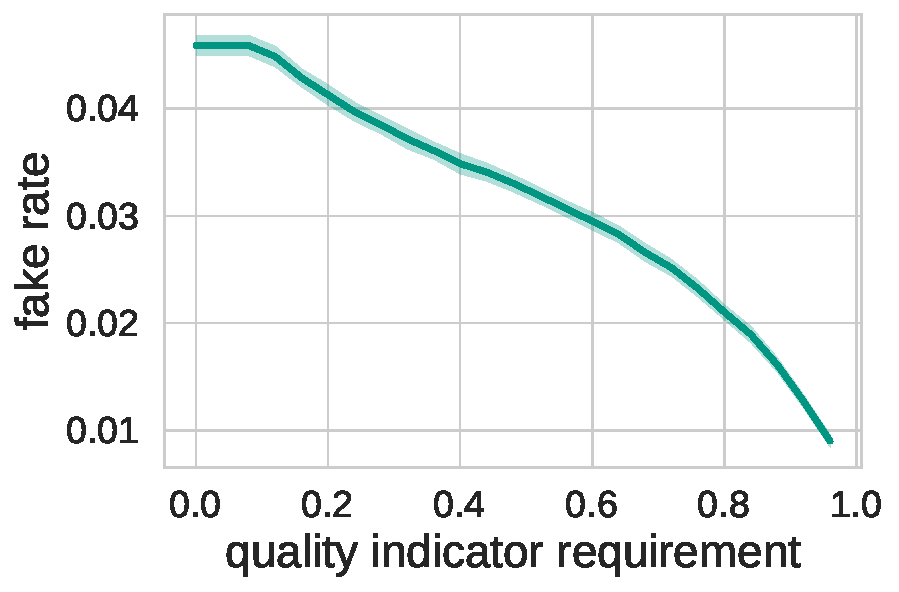
\includegraphics[width=\textwidth]{figures/cdc-qi-new/fake_rate.pdf}
    \end{column}
  \end{columns}
\end{frame}

\begin{frame} 
  \frametitle{Finding efficiency and Fake Rate for the VXD QE}
  \begin{columns}
    \begin{column}{.5\textwidth}
      \includegraphics[width=\textwidth]{figures/vxd-qi/findeff.pdf}
    \end{column}
    \begin{column}{.5\textwidth}
      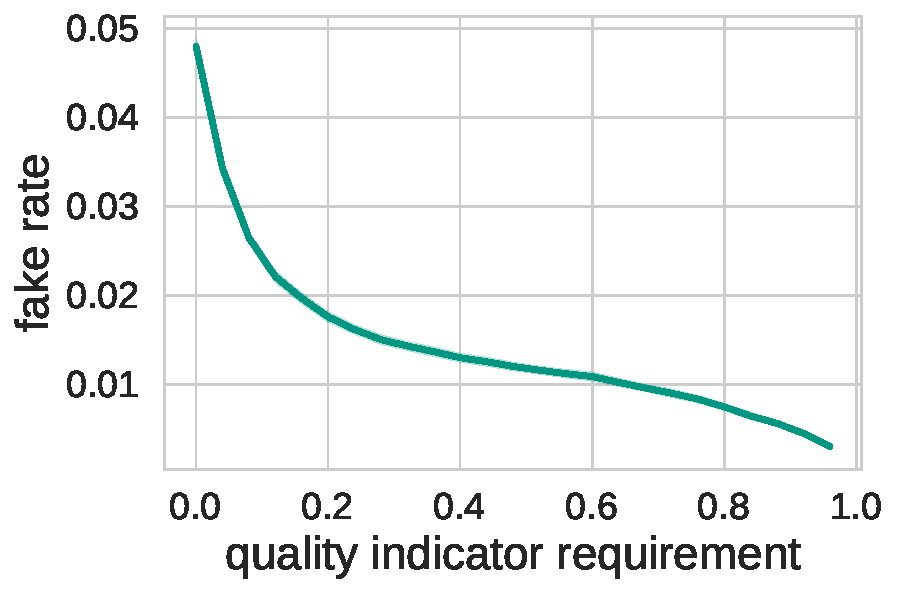
\includegraphics[width=\textwidth]{figures/vxd-qi/fake_rate.pdf}
    \end{column}
  \end{columns}
\end{frame}

\begin{frame}
  \frametitle{Combined QE Performance on Clones}
  \begin{columns}
    \begin{column}{.5\textwidth}
      \center
      \includegraphics[width=\textwidth]{figures/combined-qi/fullqi_clone_rate.pdf}
    \end{column}
    \begin{column}{.5\textwidth}
      \center
      \includegraphics[width=\textwidth]{figures/combined-qi/fullqi_clone_roc_curve.pdf}
    \end{column}
  \end{columns}
\end{frame}

\begin{frame}
  \frametitle{MVA Training Parameters}
  \begin{itemize}
  \item train on \num{5000} events ($\sim$\num{50 000} tracks) each for training and testing
  \item number of input features for combined QE: 96
    \begin{itemize}
    \item CDC QE: 20
    \item SVD QE: 27
    \end{itemize}
  \item FastBDT parameters
  \begin{itemize}
    \item 200 trees
    \item 8 levels
    \item size of random sample: \SI{50}{\percent}
    \item shrinkage: \num{0.1}
    \end{itemize}
  \end{itemize}
\end{frame}

\begin{frame}
  \frametitle{Input Features for the SVD and CDC Quality Estimators}
  \begin{block}{CDC QE input features}
    \texttt{\scriptsize adc\_max, adc\_mean, adc\_min, adc\_sum, adc\_variance, drift\_length\_max,
      drift\_length\_mean, drift\_length\_min, drift\_length\_sum, drift\_length\_variance, empty\_s\_max,
      empty\_s\_mean, empty\_s\_min, empty\_s\_sum, empty\_s\_variance, has\_matching\_segment, pt, s\_range,
      size, sz\_slope}
  \end{block}
  \begin{block}{SVD QE input features}
    \texttt{\scriptsize NSpacePoints, charge\_max, charge\_mean, charge\_min, charge\_std,
      energyLoss\_max, energyLoss\_mean, energyLoss\_min, energyLoss\_std, seedCharge\_max,
      seedCharge\_mean, seedCharge\_min, seedCharge\_std, size\_max, size\_mean, size\_min, size\_std,
      tripletFit\_Chi2, tripletFit\_PMag, tripletFit\_P\_Eta, tripletFit\_P\_Mag, tripletFit\_P\_Phi,
      tripletFit\_P\_X, tripletFit\_P\_Y, tripletFit\_P\_Z, tripletFit\_Pt, tripletFit\_QI}
  \end{block}

\end{frame}

\begin{frame}
  \frametitle{Input Features for the Combined Quality Estimator}
  \texttt{\scriptsize CDC\_FitSuccessful, CDC\_QI, Fit\_Charge, Fit\_Chi2, Fit\_NFailedPoints,
    Fit\_Ndf, Fit\_PVal, Fit\_Successful, N\_CDCRecoTracks, N\_CDC\_hits, N\_PXDRecoTracks,
    N\_PXD\_hits, N\_RecoTracks, N\_SVDRecoTracks, N\_SVD\_hits, N\_TP\_noKalmanFitterInfo,
    N\_diff\_PXD\_SVD\_RecoTracks, N\_diff\_SVD\_CDC\_RecoTracks, N\_no\_TrackPoint, N\_total\_hits,
    POCA\_Mom\_Mag, POCA\_Mom\_Phi, POCA\_Mom\_Pt, POCA\_Mom\_Theta, POCA\_Mom\_Z, POCA\_Pos\_Mag,
    POCA\_Pos\_Phi, POCA\_Pos\_Pt, POCA\_Pos\_Theta, POCA\_Pos\_Z, PXD\_QI,
    RTs\_Min\_Mom\_diff\_Mag, RTs\_Min\_Mom\_diff\_Mag\_idx, RTs\_Min\_Mom\_diff\_Pt,
    RTs\_Min\_Mom\_diff\_Pt\_idx, RTs\_Min\_Pos\_diff\_Phi, RTs\_Min\_Pos\_diff\_Phi\_idx,
    RTs\_Min\_Pos\_diff\_Theta, RTs\_Min\_Pos\_diff\_Theta\_idx, SVD\_CDC\_CDCwall\_Chi2,
    SVD\_CDC\_CDCwall\_Mom\_diff\_Eta, SVD\_CDC\_CDCwall\_Mom\_diff\_Mag,
    SVD\_CDC\_CDCwall\_Mom\_diff\_Phi, SVD\_CDC\_CDCwall\_Mom\_diff\_Pt,
    SVD\_CDC\_CDCwall\_Mom\_diff\_Theta, SVD\_CDC\_CDCwall\_Mom\_diff\_Z,
    SVD\_CDC\_CDCwall\_Pos\_diff\_Eta, SVD\_CDC\_CDCwall\_Pos\_diff\_Mag,
    SVD\_CDC\_CDCwall\_Pos\_diff\_Phi, SVD\_CDC\_CDCwall\_Pos\_diff\_Pt,
    SVD\_CDC\_CDCwall\_Pos\_diff\_Theta, SVD\_CDC\_CDCwall\_Pos\_diff\_Z,
    SVD\_CDC\_POCA\_Mom\_diff\_Eta, SVD\_CDC\_POCA\_Mom\_diff\_Mag, SVD\_CDC\_POCA\_Mom\_diff\_Phi,
    SVD\_CDC\_POCA\_Mom\_diff\_Pt, SVD\_CDC\_POCA\_Mom\_diff\_Theta, SVD\_CDC\_POCA\_Mom\_diff\_Z,
    SVD\_CDC\_POCA\_Pos\_diff\_Eta, SVD\_CDC\_POCA\_Pos\_diff\_Mag, SVD\_CDC\_POCA\_Pos\_diff\_Phi,
    SVD\_CDC\_POCA\_Pos\_diff\_Pt, SVD\_CDC\_POCA\_Pos\_diff\_Theta, SVD\_CDC\_POCA\_Pos\_diff\_Z,
    SVD\_FitSuccessful, SVD\_QI, SVD\_has\_SPTC, \_N\_tracking\_hits, seed\_Charge, seed\_Mom\_Mag,
    seed\_Mom\_Phi, seed\_Mom\_Pt, seed\_Mom\_Theta, seed\_Mom\_Z, seed\_Pos\_Mag, seed\_Pos\_Phi,
    seed\_Pos\_Pt, seed\_Pos\_Theta, seed\_Pos\_Z, seed\_Time, smoothedChi2\_firstCDChit,
    smoothedChi2\_lastSVDhit, smoothedChi2\_max, smoothedChi2\_mean, smoothedChi2\_median,
    smoothedChi2\_min, smoothedChi2\_n\_zeros, smoothedChi2\_std, weight\_firstCDChit,
    weight\_lastSVDhit, weight\_max, weight\_mean, weight\_median, weight\_min, weight\_n\_zeros,
    weight\_std}
\end{frame}

\end{document}

%%% Local Variables:
%%% coding: utf-8
%%% mode: LaTeX
%%% TeX-engine: default
%%% TeX-master: t
%%% fill-column: 100
%%% ispell-dictionary: "english"
%%% eval: (flyspell-mode 1)
%%% eval: (add-to-list 'TeX-outline-extra '("\\\\frametitle\\b" 7))
%%% End: